\subsection{Boundary Cases}
\label{Boundary Cases}

\subimport{introduction/}{introduction}
\subimport{experiment/}{experiment}

\subsubsection{Memory Boundary Results}
\label{Memory Boundary Results}
This chapter depicts the amount of memory used by the algorithms over time, especially on the boundary conditions of the experiment.

\subsubsection{Ullman Algorithm}
\begin{figure}[H]
  \begin{center}
      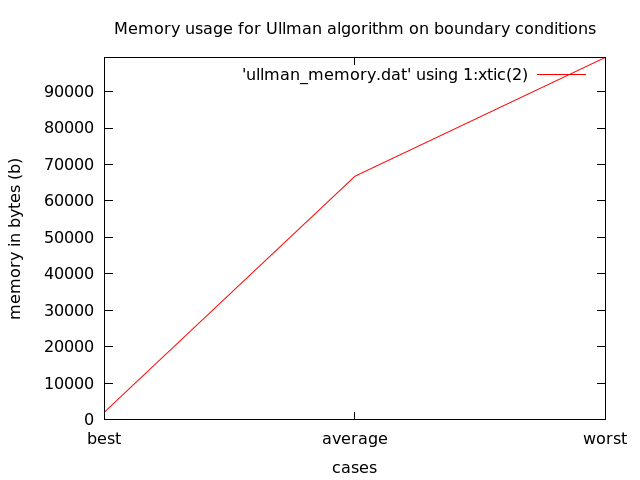
\includegraphics[width=0.8\textwidth]{ullman_memory.png}
  \end{center}    
  \caption{Representation of the memory usage by the Ullman algorithm on boundaries}
  \label{fig:case_ullman_memory}
\end{figure} 

\paragraph{Analysis of results}
Figure \ref{fig:case_ullman_memory} depicts the amount of memory used by the Ullman algorithm over time. The figure indicated that the amount of memory used
by the algorithm increases at a steady from the defined best case to the worst case for some graph $G$.\newline\newline
Based on the results from figure \ref{fig:case_ullman_memory}, it is clear that the algorithm consumes more of the systems RAM on the worst of the extreme case
and the most little of RAM in the best of such cases.

\subsubsection{VF2 Algorithm}
\begin{figure}[H]
  \begin{center}
      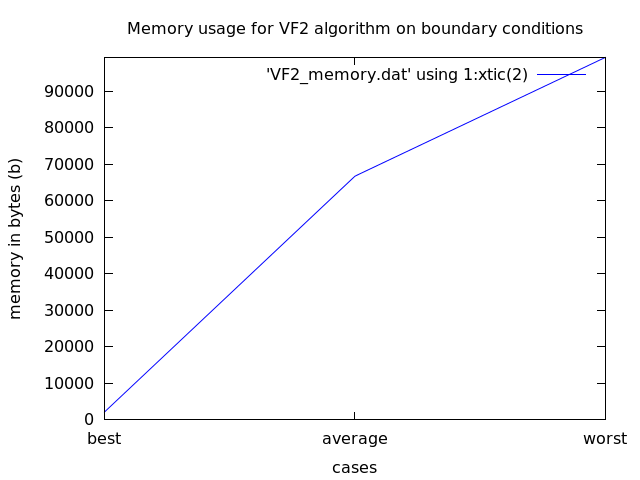
\includegraphics[width=0.8\textwidth]{vf2_memory.png}
  \end{center}    
  \caption{Representation of the memory usage by the VF2 algorithm on boundaries}
  \label{fig:case_vf2_memory}
\end{figure} 

\paragraph{Analysis of results}
Figure \ref{fig:case_vf2_memory} depicts that amount of memory used by the VF2 algorithm during the execution of the graph matching procedure of the VF2 
algorithm over time. The figure demonstrates the memory consumption characteristics of the algorithm on the defined boundary conditions.\newline\newline
Based on the results from \ref{fig:case_vf2_memory}, we can see that the amount of memory used by the VF2 algorithm, much like the Ullman algorithm also 
increases overtime.

\subsubsection{Conclution}
The memory consumption characteristics demonstrated in figures \ref{fig:case_ullman_memory} and \ref{fig:case_vf2_memory} respectively have similary 
characteristics. The characteristic being that both algorithms seem to use very little amount of memory for the best case of the boundaries, but as the
case of the boundaries becomes gradually worse, the more memory is required by both algorithms.\newline\newline
Apart from the foremention characteristic, another observation that is made is that the memory used by the algorithms seems to be arbitrarily similary 
for each instance of their respective executions. \newline\newline
\textbf{Best:} condition, the Ullman algorithm uses 2136 bytes of memory and so does the VF2 algorithm.\newline\newline
\textbf{Average:} case, the Ullman algorithm uses 66780 bytes and the VF2 algorithm uses 66784 bytes.\newline\newline 
\textbf{Worst:} case, Ullman uses 99344 and VF2 uses 99340 bytes. Thus it can be concluded from this observation that with regards to the memory used, the two algorthms are arbitrarily similar in
that regards.

\newpage

\subsubsection{Time Boundary Results}
\label{Time Boundary Results}
This chapter depicts the amount of time taken by the algorithms in order to successfully complete the graph matching procedure, especially on the 
boundary conditions of the experiment.

\subsubsection{Ullman Algorithm}
\begin{figure}[H]
  \begin{center}
      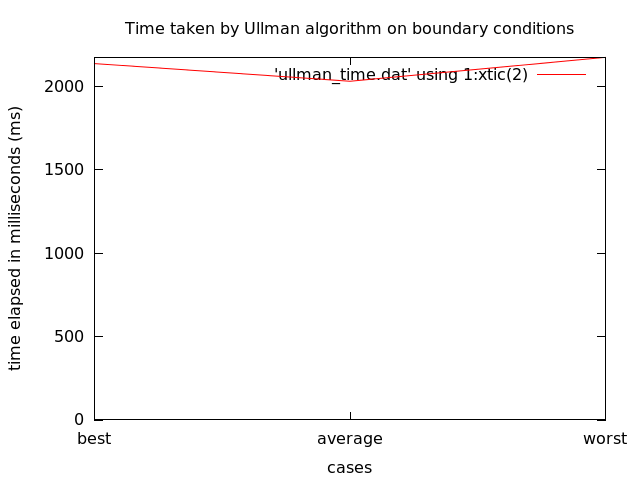
\includegraphics[width=0.8\textwidth]{ullman_time.png}
  \end{center}    
  \caption{Representation of the time taken by the Ullman algorithm on boundaries}
  \label{fig:case_ullman_time}
\end{figure} 

\paragraph{Analysis of results}
Figure \ref{fig:case_ullman_time} demonstrates the amount of time taken by the Ullman algorithm to successfully complete its graph matching procedure.
From figure \ref{fig:case_ullman_time}, we can see that the Ullman algorithm is extremely resource intensive will regards to the time it takes. Even in the 
\textbf{best}, the algorithm takes a relatively long time to complete its execution.\newline\newline
A secondary observation made from \ref{fig:case_ullman_time} is that, though the time values are high, they do appear to show very little flactuations, and are thus steady.

\subsubsection{VF2 Algorithm}
\begin{figure}[H]
  \begin{center}
      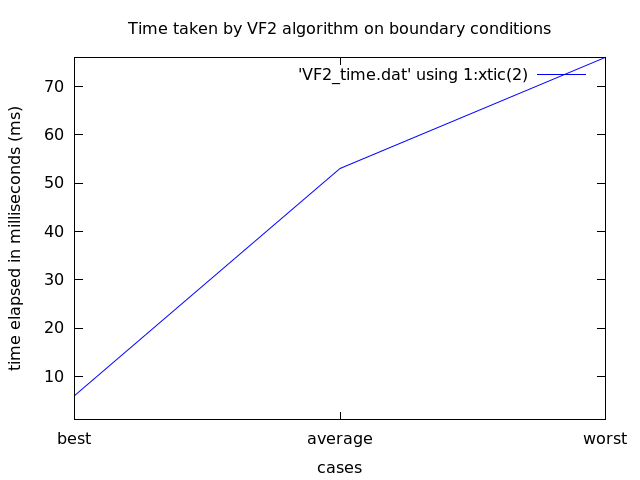
\includegraphics[width=0.8\textwidth]{vf2_time.png}
  \end{center}    
  \caption{Representation of the time taken by the Ullman algorithm on boundaries}
  \label{fig:case_vf2_time}
\end{figure} 

\paragraph{Analysis of results}
Figure \ref{fig:case_vf2_time} depicts the amount of time taken by the VF2 algorithm to successfully complete its graph matching procedure.
From figure \ref{fig:case_vf2_time}, it is clear that the amount of time taken to successfully complete the matching procedure increases over time, and the 
increase seems to be constant, from the \textbf{best} case to the worst.

\subsubsection{Conclution}
The Ullman and VF2 algorithms demonstrate very different behaviours with regards to the amount of time take to complete their respective matching procedures.\newline\newline
The Ullman algorithm requires a much larger amount of time for its completion, even in the \textbf{best} case, where the time required is 2136 ms.\newline\newline
The VF2 algorithm however, requires very little time relative to the Ullman algorithm, especially in the best case, as oppose to the Ullman algorithm. The 
time required by the algorithm does increase as the cases worsen, and based on figure \ref{fig:case_vf2_time},we can see that the increase is relatively constant.\newline\newline
By analysing the time requirements of both algorithms, we can safely deduce that the VF2 algorithm is castly more efficient than the Ullman algorithm in terms 
of the amount of time required to complete the graph matching procedure. The values for each case indicating this fact are demonstrated in the table below.

\begin{table}[h]
\centering
\caption{Time values for Ullman algorithm vs. VF2 algorithm}
\label{my-label}
\begin{tabular}{|l|l|l|}
\hline
Case    & \multicolumn{2}{l|}{Algorithm} \\ \hline
        & Ullman          & VF2          \\ \hline
Best    & 2136            & 6            \\ \hline
Average & 2030            & 53           \\ \hline
Worst   & 2173            & 76           \\ \hline
\end{tabular}
\end{table}